\begin{center}
\Huge
Forberedelse til prøve
\end{center}

\subsection*{Opgave 1}

Afgør for følgende sammenhænge mellem $x$ og $y$ om de er ligefrem eller omvendt proportionale.
\begin{align*}
	&a) \ y\cdot x = 5 &&b) \  y = -4x   \\
	&c) \ \frac{y}{x} = 2  &&d) \ y = \frac{6}{x}   
\end{align*}


\subsection*{Opgave 2}

For følgende funktioner $f$ og $g$ bestem da den sammensatte funktion $f(g(x))$. 

\begin{align*}
	&a) \  f(x) = x^2 \textnormal{ og } g(x) = 2x+1\\
	&b) \  f(x) = \sqrt{x} \textnormal{ og } g(x) = 4x-3\\
	&c) \  f(x) = \ln(x) \textnormal{ og } g(x) = \sqrt{x}\\
	&d) \  f(x) = x^4 \textnormal{ og } g(x) = x^3\\
\end{align*}

\subsection*{Opgave 3}

En stykvist defineret funktion er defineret ved
\begin{align*}
	f(x) = 
	\begin{cases}
		\sqrt{x}, &\textnormal{ hvis } x \geq 0,\\
		x^2-2x+1, &\textnormal{ hvis } x < 0.		
	\end{cases}
\end{align*}

\begin{enumerate}[label=\roman*)]
	\item Tegn grafen for $f$ på intervallet $[-4,4]$.
	\item Bestem $f(4)$.
\end{enumerate}

\subsection*{Opgave 4}

Bestem graden for følgende polynomier.

\begin{align*}
	&1) \ x^2+4x+1   &&2) \ x^5-2x^2    \\
	&3) \ -4x^3+5x^7   &&4) \  x^2+2x^3+3x^4+4x^5+5x^6    \\
\end{align*}

\subsection*{Opgave 5}

Andengradspolynomierne $f$ og $g$ har henholdsvis parablerne $A$ og $B$, som kan ses på Figur \ref{fig:parabler}.
\begin{figure}[H]
	\centering
	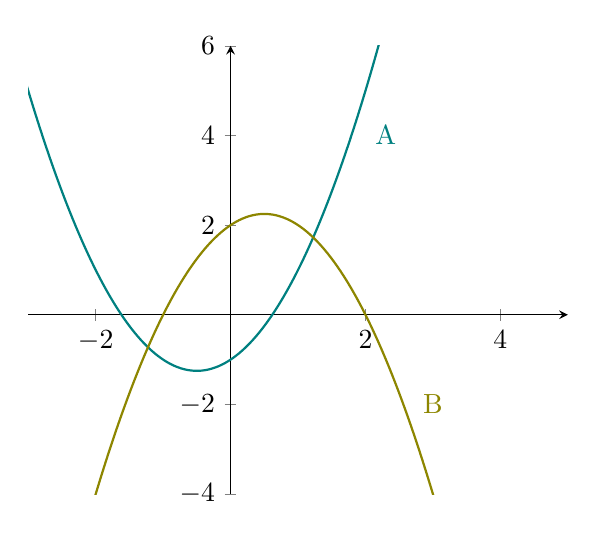
\begin{tikzpicture}
		\begin{axis}[
		axis lines = center,
		xmin = -3, xmax = 5,
		ymin = -4, ymax = 6
		]
			\addplot[color = teal, samples = 200, thick] {x^2+x-1};
			\addplot[color = olive, samples = 200, thick] {-x^2+x+2};
			\node[color = olive] at (axis cs: 3, -2) {B};
			\node[color = teal] at (axis cs:2.3,4) {A};
		\end{axis}
	\end{tikzpicture}
	\caption{Parablerne $A$ og $B$}
	\label{fig:parabler}
\end{figure}

\begin{enumerate}[label=\roman*)]
	\item Bestem $c$-værdien for $f$ og $g$.
	\item Bestem fortegnet på $a$- og $b$-værdierne for $f$ og $g$
	\item Bestem fortegnet på diskriminanten for $f$ og $g$.
	\item Bestem rødderne for $g$.
\end{enumerate}

\subsection*{Opgave 6 (Uden Maple)}
Et polynomium $f$ er givet ved
\begin{align*}
	f(x) = 12 + 2 x - 2 x^2
\end{align*}
\begin{enumerate}[label=\roman*)]
	\item Bestem $f(2)$
	\item Bestem rødderne for $f$
\end{enumerate}


\subsection*{Opgave 7 (Uden Maple)}

Løs følgende ligninger

\begin{align*}
	&a) \ x^2 + 2x = 3 \ &&b) \ -x^2 = 6x + 8 
\end{align*}

\subsection*{Opgave 8}

I \href{https://github.com/ChristianJLex/TeachingNotes/raw/master/2023-2024/Data og lign/Polynomisk.xlsx}{\color{blue!60} dette datasæt} fremgår en række datapunkter.
\begin{enumerate}[label=\roman*)]
	\item Brug residualplots til at afgøre, hvilken polynomisk regression, der bedst beskriver 
	datasættet.
	\item Anvend regression på datasættet med den valgte regression
	\item Bestem $f(9)$.
	\item Bestem rødderne for $f$. 
\end{enumerate}